% General match
\DeclareMathOperator*{\argmax}{arg\,max}
\DeclareMathOperator*{\argmin}{arg\,min}
\newcommand{\mli}[1]{\mathit{#1}}
\newcommand{\concat}[0]{{\cdot}}
\newcommand{\bp}{\,bp} %\newcommand{\bp}{\unit{\,bp}}
\newcommand{\kbp}{\,kbp} %\newcommand{\kbp}{\unit{\,kbp}}
\newcommand{\qty}[2]{#1\ #2} % TODO: remove \qty and \unit in favor of siunitx
\newcommand{\unit}[1]{#1} 
\newcommand{\Oh}[0]{O}
\newcommand{\ed}[0]{\mbox{ed}\xspace}
\newcommand{\st}[2]{\langle #1, #2 \rangle}

% Edit costs
\newcommand{\Costs}[0]{\mathbb{R}_{\geq 0}}
\newcommand{\costcap}[0]{c}
\newcommand{\cedits}[0]{\Delta}
\newcommand{\cmatch}[0]{\Delta_\text{match}}
\newcommand{\csubst}[0]{\Delta_\text{subst}}
\newcommand{\cins}[0]{\Delta_\text{ins}}
\newcommand{\cdel}[0]{\Delta_\text{del}}
\newcommand{\dist}[0]{\mli{ED_\Delta}}
\newcommand{\maxdel}[0]{n_\text{del}}
\newcommand{\maxins}[0]{n_\text{ins}}

% Graph terms
\newcommand{\g}{g^*\!}
\newcommand{\h}{h^*\!}
\newcommand{\A}[0]{A$^\star$\xspace}
\newcommand{\Path}{\pi^*}
% reference graph
\newcommand{\reference}[1]{#1_\texttt{r}}
\newcommand{\RG}[0]{\reference{G}}
\newcommand{\RGV}[0]{\reference{V}}
\newcommand{\RGE}[0]{\reference{E}}
% trie
\newcommand{\trie}[1]{#1_\texttt{r}^\texttt{+}}
\newcommand{\TG}[0]{\trie{G}}
\newcommand{\TGV}[0]{\trie{V}}
\newcommand{\TGE}[0]{\trie{E}}
% edit graph
\newcommand{\edit}[1]{#1_\texttt{e}}
\newcommand{\EG}[0]{\edit{G}}
\newcommand{\EGV}[0]{\edit{V}}
\newcommand{\EGE}[0]{\edit{E}}
% alignment graph
% TODO: simplify to just G(V,E)
%\newcommand{\alignment}[2][q]{#2_\texttt{a}^{#1}}
\newcommand{\alignment}[2][q]{#2}
\newcommand{\AG}[1][q]{\alignment[#1]{G}}
\newcommand{\AGV}[1][q]{\alignment[#1]{V}}
\newcommand{\AGE}[1][q]{\alignment[#1]{E}}

% Seed heuristic
\newcommand{\csh}[0]{chaining seed heuristic\xspace}
\newcommand{\Csh}[0]{Chaining seed heuristic\xspace}
\newcommand{\CSH}[0]{CSH\xspace}
\newcommand{\sh}[0]{seed heuristic\xspace}
\newcommand{\Sh}[0]{Seed heuristic\xspace}
\newcommand{\SH}[0]{SH\xspace}
\newcommand{\seeds}{\mathcal S}
\newcommand{\matches}{\mathcal M}
\newcommand{\Pot}{P}
\newcommand{\spot}{r}
\newcommand{\cost}{\operatorname{cost}}
\newcommand{\matchscore}{\operatorname{score}}
\newcommand{\seedscore}{\operatorname{score}}
\newcommand{\statescore}{S}
\newcommand{\chainscore}{S_{\mathrm{chain}}}
\newcommand{\shscore}{S_{\mathrm{sh}}}
\newcommand{\cshscore}{S_{\mathrm{csh}}}

\newcommand{\seedh}[0]{\mbox{seed heuristic}\xspace}
\newcommand{\prefixh}[0]{\mbox{prefix heuristic}\xspace}
\newcommand{\trieroot}{\ensuremath{\mli{root}}}

% Seed heuristic with pruning
\newcommand{\ssh}{_{\mathrm{sh}}}
\newcommand{\scsh}{_{\mathrm{csh}}}
\newcommand{\hsh}{h\ssh\!}
\newcommand{\hcsh}{h\scsh\!}
\newcommand{\hshM}{h\ssh^\matches\!}
\newcommand{\hcshM}{h\scsh^\matches\!}
\newcommand{\hh}{\hat h}
\newcommand{\hshS}{\hat h\ssh\!}
\newcommand{\hcshS}{\hat h\scsh\!}

\newcommand{\layer}{\mathcal L}
\newcommand{\start}{\operatorname{start}}
\newcommand{\substr}[3]{#1_{#2{\dots}#3}}
\renewcommand{\path}[2]{(#1{\leadsto}#2)}

% Global alignment
% Fig.2
\newcommand{\bluecircle}{
\includegraphics[height=4pt]{imgs/fig2-symbols/blue-circle.pdf}}
\newcommand{\greencircle}{
\includegraphics[height=4pt]{imgs/fig2-symbols/green-circle.pdf}}
\newcommand{\cross}{
\includegraphics[height=4pt]{imgs/fig2-symbols/cross.pdf}}
\newcommand{\seed}{
\includegraphics[width=6pt]{imgs/fig2-symbols/seed.pdf}}
\newcommand{\match}{
\includegraphics[height=4pt]{imgs/fig2-symbols/match.pdf}}
\newcommand{\redcolumn}{
\includegraphics[height=5pt]{imgs/fig2-symbols/red-column.pdf}}
\newcommand{\greencolumn}{
\includegraphics[height=5pt]{imgs/fig2-symbols/green-column.pdf}}
% Fig.3
\newcommand{\bluesquare}{
\includegraphics[height=4pt]{imgs/fig3-symbols/bluesquare.pdf}}
\newcommand{\greensquare}{
\includegraphics[height=4pt]{imgs/fig3-symbols/greensquare.pdf}}
\newcommand{\blackmatch}{
\includegraphics[height=5pt]{imgs/fig3-symbols/blackmatch.pdf}}
\newcommand{\redmatch}{
\includegraphics[height=5pt]{imgs/fig3-symbols/redmatch.pdf}}
% Plots
\newcommand{\edlibsymbol}{
\includegraphics[height=4pt]{imgs/plots-symbols/edlib.pdf}}
\newcommand{\wfasymbol}{
\includegraphics[height=4pt]{imgs/plots-symbols/wfa.pdf}}
\newcommand{\shsymbol}{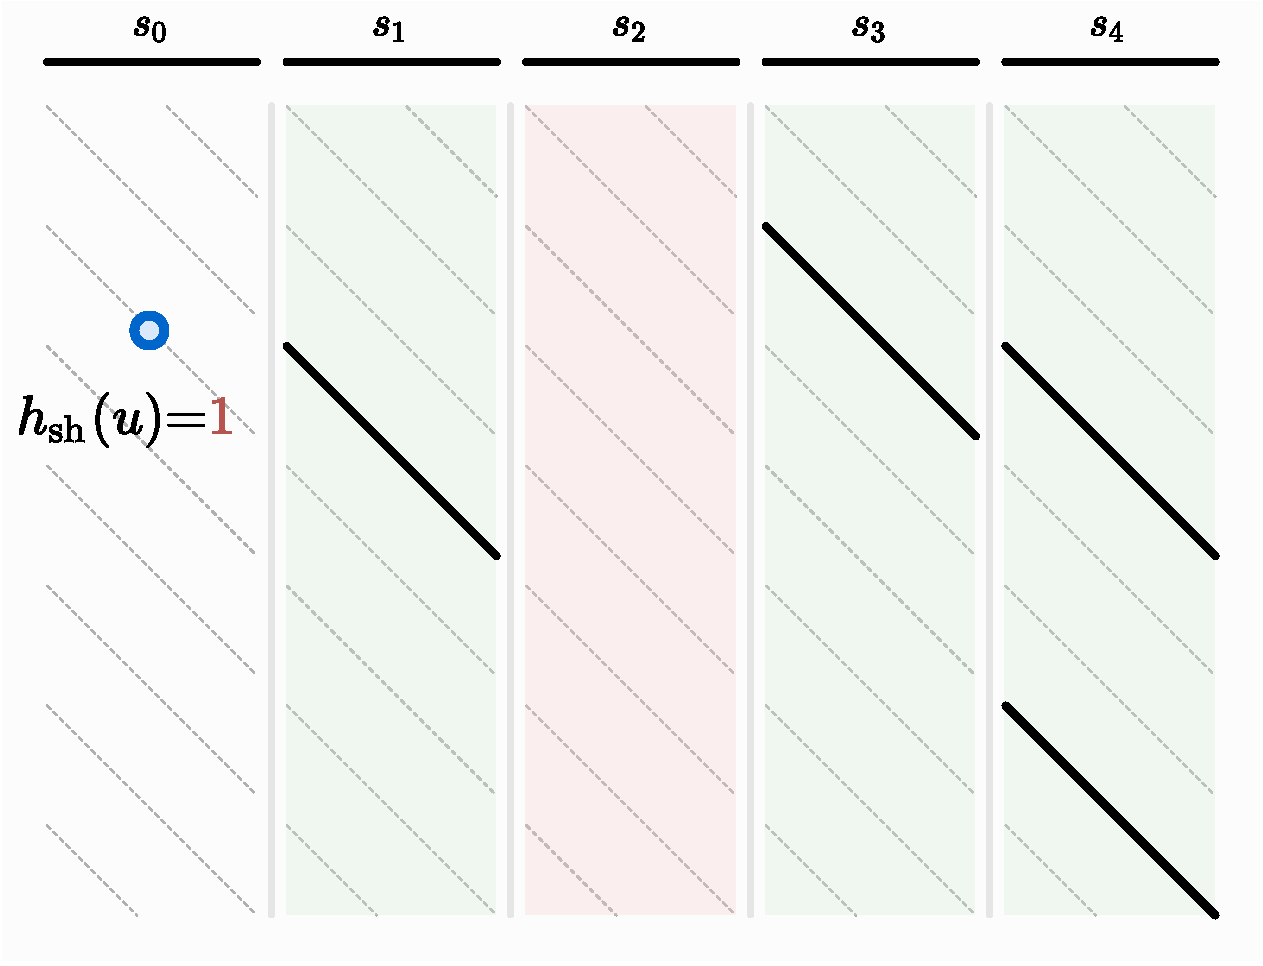
\includegraphics[height=4pt]{imgs/plots-symbols/sh.pdf}}
\newcommand{\shsymbolsq}{
\includegraphics[height=4pt]{imgs/plots-symbols/sh-down.pdf}}
\newcommand{\cshsymbol}{
\includegraphics[height=4pt]{imgs/plots-symbols/csh.pdf}}
\newcommand{\cshsymbolsq}{
\includegraphics[height=4pt]{imgs/plots-symbols/csh-down.pdf}}

% Seeds paper
% crumbs icons
\newcommand{\bluecrumb}{%
  \begingroup\normalfont
  \includegraphics[height=\fontcharht\font`\B]{figures/blue-square.pdf}%
  \endgroup
}
\newcommand{\greencrumb}{%
  \begingroup\normalfont
  
\includegraphics[height=1.1\fontcharht\font`\B]{figures/green-square.pdf}%
  \endgroup
}
\newcommand{\yellowcrumb}{%
  \begingroup\normalfont
  
\includegraphics[height=1.1\fontcharht\font`\B]{figures/yellow-triangle.pdf}%
  \endgroup
}
\newcommand{\violetcrumb}{%
  \begingroup\normalfont
  
\includegraphics[height=\fontcharht\font`\B]{figures/violet-circle.pdf}%
  \endgroup
}
% other icons
\newcommand{\greentick}{%
  \begingroup\normalfont
  
\includegraphics[height=\fontcharht\font`\B]{figures/green-tick.pdf}%
  \endgroup
}

% Mapping tools
\newcommand{\dijkstra}[0]{\mbox{Dijkstra}\xspace}
\newcommand{\astarix}[0]{\mbox{\textsc{AStarix}}\xspace}
\newcommand{\astarixseeds}[0]{\mbox{\textsc{AStarix-seeds}}\xspace}
\newcommand{\astarixprefix}[0]{\mbox{\textsc{AStarix-prefix}}\xspace}
\newcommand{\astarixurl}[0]{\url{https://github.com/eth-sri/astarix}\xspace}
\newcommand{\astarixurlwithbranch}[0]{\url{https://github.com/eth-sri/astarix/tree/recomb2020}\xspace}
\newcommand{\graphaligner}[0]{\textsc{GraphAligner}\xspace}
\newcommand{\bitparallel}[0]{\textsc{BitParallel}\xspace}
\newcommand{\brownie}[0]{\textsc{BrownieAligner}\xspace}
\newcommand{\pasgal}[0]{\textsc{PaSGAL}\xspace}
\newcommand{\vg}[0]{\textsc{VG}\xspace}
\newcommand{\valigntool}[0]{\textsc{V-ALIGN}\xspace}
\newcommand{\vargas}[0]{\mbox{\textsc{Vargas}}\xspace}
\newcommand{\hga}[0]{\mbox{\textsc{HGA}}\xspace}
\newcommand{\art}[0]{\mbox{\textsc{ART}}\xspace}
\newcommand{\randomreads}[0]{\mbox{\textsc{randomreads.sh}}\xspace}

% Global alignment tools
\newcommand{\difftool}[0]{\mbox{\textsc{diff}}\xspace}
\newcommand{\edlib}[0]{\mbox{\textsc{Edlib}}\xspace}
\newcommand{\oldwfa}[0]{\mbox{\textsc{WFA}}\xspace}
\newcommand{\wfa}[0]{\mbox{\textsc{BiWFA}}\xspace}
\newcommand{\seqan}[0]{\mbox{\textsc{SeqAn}}\xspace}
\newcommand{\parasail}[0]{\mbox{\textsc{Parasail}}\xspace}
\newcommand{\astarpa}[0]{\mbox{\textsc{A*PA}}\xspace}
%\newcommand{\lcs}[0]{\mbox{LCS}\xspace}
%\newcommand{\lcskpp}[0]{\mbox{LCSk++}\xspace}

% Datasets
\newcommand{\datasetOne}{CHM13}
\newcommand{\datasetTwo}{NA12878}